
In this chapter, a numerical simulation able to replicate the most common breast compression techniques was developed. This tool is used to compare different breast compression paddles considering the patient experience as well as the image quality and average glandular dose. The breast biomechanical model described  in Chapter \ref{chapter:myBioMecaModel} was used to create two different breast models corresponding to the two involved volunteers. To simulate breast compression, finite element models of standard paddles were developed and put in contact with the two breast models.

First, a comparative study was performed between various paddle designs. The compression of the right breast of both volumes was simulated with flex and rigid paddles. We proposed to quantify the perceived pain for a given paddle design through three entities, namely contact pressure, internal stress and strain distributions. After compression, a set of virtual macrocalcifications were inserted into the breast volumes. A Monte-Carlo based simulation mimicking the acquisition of images with a mammography system was applied to the breast volumes. Then, the imaging performance was assessed by measuring the signal-difference-to-noise-ratio (SDNR), the signal-to-noise-ratio (SNR) and the average glandular dose (AGD).

Finally, the compression mechanics was analyzed as a function of breast positioning. To this end, the breast geometry of the second volunteer was compressed with different paddle positions with respect to the chest wall. The patient comfort was assessed for three paddle positions. 

 

\clearpage


\section{Breast compression modeling}
In Chapter \ref{chapter:myBioMecaModel} a new biomechanical breast model was proposed. An optimization process was developed allowing to determine subject-specific breast stress-free geometry and the corresponding mechanical properties. At this stage, the exhaustive semi-automatic search of the constitutive parameters is computationally expensive to perform. Therefore, because of lack of time, the model calibration was carried out for the first volunteer only. However, to perform a qualitative study comparing different paddle models, data of more than one subject is needed. To provide our study with a larger data set, the biomechanical breast model of the second volunteer was created without performing the model calibration to the subject specific mechanical properties. This model represents a new realistic breast geometry with a larger volume and different tissues mechanical behavior which will not characterize the actual breast mechanics of the second volunteer.

To simulate breast compression, finite element models of compression paddles were developed. The realism of these simulations was evaluated by comparing the resulting breast thickness and the applied force to the corresponding data measured during the most recent mammograms of both volunteers. The resulting mechanical response revealed the limitations of a Neo-Hookean strain energy function and the necessity of updating  the tissues constitutive models. 

In the following section, first the designed compression paddles were introduced. Then, the compression mechanics as simulated using the biomechanical breast model are described. Accordingly,  the constitutive models of breast tissues were reviewed and a new form of the strain energy density function was proposed.  

\subsection{FE modeling of compression paddles}
In this study, standard paddles (standard rigid and flex paddles) generally used for regular screening were considered. Only one paddle geometry was modeled based on the technical specifications from a Senographe Pristina mammography unit. Three different paddle models were created.  

First, the paddle flexibility due to its material properties was neglected. The rigid paddle model (RPM\nomenclature{RPM}{Rigid Paddle Model}) was therefore defined as a fully rigid body with only one translational degree of freedom in the downward direction. 

Then, for the flex paddle model (FPM\nomenclature{FPM}{Flex Paddle Model}), a rotation around the longitudinal axis was added. The additional degree of freedom was modeled using a rotational-only joint type of element. The joint stiffness was computed by fitting the force-deflection curve of a standard flex paddle measured on a Senographe Pristina unit. For this, a rigid plate was fixed perpendicularly to the image receptor at its external edge, in order to block the SFP translation degree of freedom (Figure \ref{fig:deflectionangle}.a). To ensure the paddle rotation around the $Oy$ axis only, the rigid plate was chosen to have the same length (in $Oy$ direction) as the compression paddle. The deflection angle was measured using a digital inclinometer ($\pm0.1$\textdegree  accuracy). The paddle was lowered progressively, such as the deflection angle was incremented by steps of $0.5$\textdegree, until the maximal recommended compression force was reached ($F=200N$). At each step, the compression force was read from the calibrated mammography unit. The experiment was repeated 3 times. The relation between the mean compression force and the deflection angle is shown in Figure \ref{fig:deflectionangle}.b. An estimated second-degree polynomial was used to define the joint stiffness for the FE analysis.

\begin{figure}[!h]
\centering
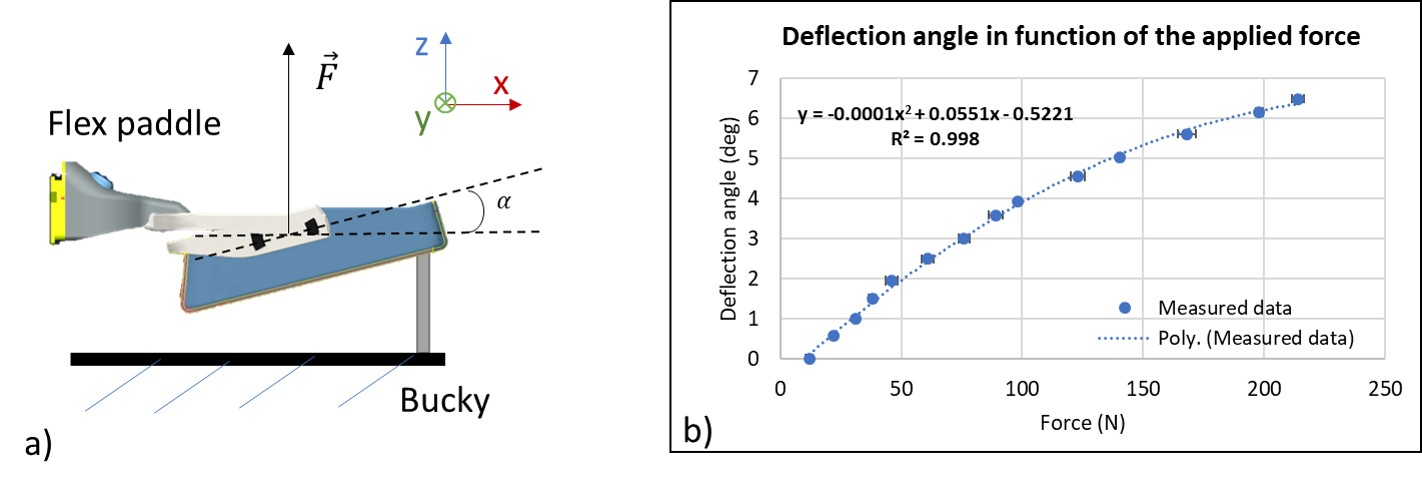
\includegraphics[width=0.9\textwidth,keepaspectratio]{figures/deflectionAngle.jpg} 
\caption{ a) Experiment set-up, b) Deflection angle as function of the applied force }\label{fig:deflectionangle}
\end{figure}

As concerns the third paddle model, namely the elastic paddle model (EPM\nomenclature{EPM}{Elastic Paddle Model}), the deflection due to the material properties was included. The paddle thickness was set to $4mm$ and it assumed to be made of Lexan material ($\lambda_{lexan}= 2250 \ MPa$ and $\nu_{lexan}= 0.4$).   Only one translational degree of freedom in the downward direction was considered. The paddle was modeled using shell elements. 

For the three paddle models, the interaction between the compression paddles and the breast was modeled using a frictionless contact. The penalty algorithm was used with a penetration factor equal to 0.1 and a contact stiffness equal to 1. 
 
\subsection{Breast compression mechanics}

The realism of breast compression simulations was verified by confrontation with real data. The positioning and compression of a small breast, like the one we have for the first volunteer, may be complex. Sometimes the technologist has to hold the breast between the image receptor and the paddle until the compression force is high enough to preclude the breast from sliding outside of the image receptor field of view. This difficulty is also present in a simulation framework, especially since we do not simulate the breast positioning gesture by the radiologist. To facilitate the compression process during the evaluation step, it was therefore decided to use only the larger breast geometry  provided by the second volunteer.

In a clinical framework, woman breasts are compressed in an up-right or prone body positions. Under compression, the gravity induced tissues pre-stresses can be neglected when compared to the compression-induced stresses \citep{han_development_2012, ruiter_model_based_2006, sturgeon_finite_element_2016}.  Therefore, the prone breast configuration was used as the reference configuration, neglecting the tissues internal pre-stresses due to gravity loading. The breast compression was simulated using the rigid and flex paddle models. 

Prior to breast compression simulations, the breast biomechanical model corresponding to the geometry of the second volunteer in prone configuration was developed. The optimization problem estimating the set of constitutive parameters is expensive in terms of the computation time.  Therefore, for this chapter, we decided to replace the tissues constitutive parameters of the second volunteer, with the ones found in the literature  \citep{han_nonlinear_2014,  rajagopal_modelling_2007, gefen_mechanics_2007}. The corresponding equivalent modulus for each involved tissue was chosen to be the following: $\lambda_{breast}=0.5 kPa$, $\lambda_{muscle}= 10kPa$, $\lambda_{skin}=10kPa$, $\lambda_{fascia}= 160kPa$.  Of course, with this assumption, this new biomechanical model does not properly represent the breast mechanics of the second volunteer.  However, it provides a realistic model with a larger breast volume and with stiffer breast tissue which may be used in a comparative study between various compression strategies.     

The cranio-caudal incidence was modeled by positioning the image receptor at the inframammary ligament level while the paddle compresses the breast by a downward movement. The compression was stopped when the target breast thickness was reached. Such target thickness was given by the data recorded during the most recent mammogram of the second volunteer (Table \ref{tab:forceandthichnessdata}). Figure \ref{fig:thicknessforcerelationNH} shows the breast thickness as function of the applied force for the flex and the rigid paddles. The breast thickness for the flex and the rigid paddles was considered constant along $Oy$ axis. For a rigid paddle, the distance between the paddle and the image receptor was used to assess the breast thickness, and was named $h_r$  (Figure \ref{fig:thicknessforcerelationNH}). Concerning the flex paddle, the distance between the image receptor and the paddle was measured at two distinct points, first at the nipple level (named $h_1$ in Figure \ref{fig:thicknessforcerelationNH}) and the second at the breast base (named $h_2$ in Figure \ref{fig:thicknessforcerelationNH}). Therefore, the breast thickness for the flex paddle (named $h_f$ on Figure \ref{fig:thicknessforcerelationNH}) is given by the mean value of $h_1$ and $h_2$. 
 
\begin{figure}[!h]
\centering
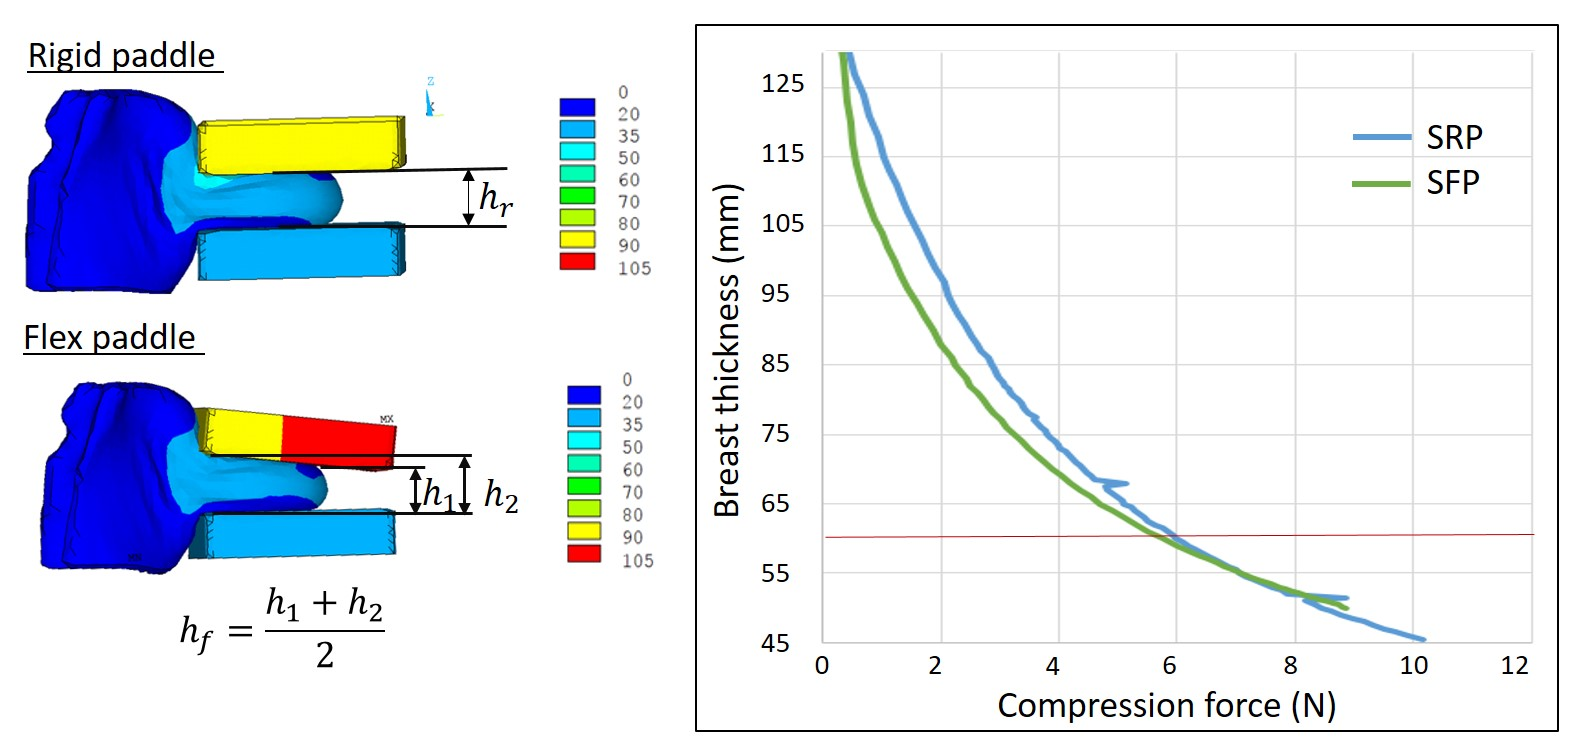
\includegraphics[width=0.9\textwidth,keepaspectratio]{figures/compressionforceNH.jpg} 
\caption{Breast flattening curve as function of the applied force for a Neo-Hookean strain energy function. SRP - standard rigid paddle, SFP -standard flex paddle}\label{fig:thicknessforcerelationNH}
\end{figure}

Several irregularities can be observed over the curve  describing the force-thickness relation when the breast is compressed with a rigid paddle. These numerical artifacts are due to inherent finite elements discretization errors.  One can see that, the total compression force at the target breast thickness ($50mm$) is about 10 times lower than the force measured during the volunteer's last mammography ($8N$ versus $94.8N$). Even if the chosen constitutive models were not accurately adapted to the patient mechanical properties, a force of $6N$ remains too low when compared to the standard compression force of $120N$ \citep{chida_reduced_2009}. Usually, a larger force is applied when compressing such large breast volumes as the one of the second volunteer.  Several compressions were tested (e.g. paddle closer to the juxtathoracic area, frictional contact with different friction coefficient) without observing any significant increase of the compression force. 

An analysis of the literature revealed that the constitutive parameters used to model breast compression are usually higher than the ones used to model the breast deformation under gravity loading. For example, Sturgeon and colleagues \citep{sturgeon_finite_element_2016} have estimated the tissues deformation under compression considering the initial shear modulus for a Neo-Hookean strain energy function equal to $\mu_{skin} = 88kPa$, $\mu_{adipose} = 1kPa$ and $\mu_{glandular}= 10kPa$. Moreover, our simulations did not demonstrate the asymptotic behavior of the compression force versus breast thickness, as described by Groot et al. \citep{de_pain_2015}.  One can conclude that, for high strains, the soft tissues undergo a stiffening process more rapidly than the stiffening as described by a Neo-Hookean law.

The limitation of the Neo-Hookean model to capture the mechanical response of some nonlinear materials is well known \citep{kaliske_finite_1997}. For large strain rates, the Neo-Hookean material may undergo a relaxation and thus become easier to deform. Therefore, another strain energy model has to be considered for the modeling of breast compression.

\subsection{Gent strain energy function}
Giving that the Neo-Hookean strain energy function provides a poor estimation for large strains, the Gent strain energy function (see Section \ref{subsection:constitutivemodels}.a)  could be used as an alternative model. The Gent function is characterized by three parameters ($\mu$, $K$, and $J_m$). For small strains, it is resumed to the Neo-Hookean model \citep{chagnon_comparison_2004}. For large strains, the $J_m$ parameter acts as a stiffening parameter and defines the upper limit of the first invariant of the left Cauchy-Green deformation tensor (Figure \ref{fig:GentvsNeoStrain}.a).  When $J_m \longrightarrow \infty$, the Gent model is reduced to the Neo-Hookean model even for large strains (Figure \ref{fig:GentvsNeoStrain}.a).  
 
\begin{figure}[!h]
\centering
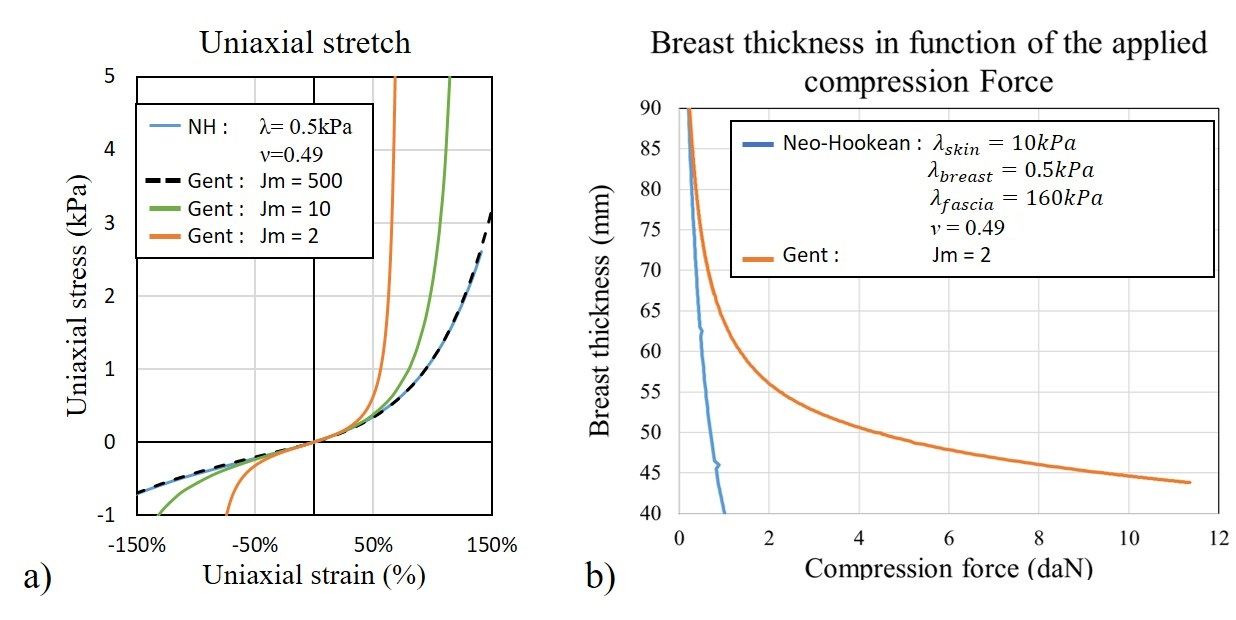
\includegraphics[width=1\textwidth,keepaspectratio]{figures/GentvsNeoStrain.jpg} 
\caption{a) Stress-strain relation for Neo-Hookean and Gent energy functions; b) Breast flattening curve as function of the applied force for a Gent energy function.}
\label{fig:GentvsNeoStrain}
\end{figure}

These properties are particularly interesting for our simulation framework. In Chapter \ref{chapter:myBioMecaModel}, the material properties have been estimated and validated for multi-loading gravity simulations. Therefore, the tissues mechanical behavior is well estimated for relatively small strains. The strain range due to breast compression is significantly larger than the one due to gravity loading. In this respect, the $J_m$ parameter may be estimated such that, for relative small strains, the Gent model remains equivalent to the Neo-Hookean model. However for larger strains,  the energy function will behave asymptotically to approach a compression force equivalent to the standard compression force (Figure \ref{fig:GentvsNeoStrain}.b). Then, only the third parameter of the energy function has to be estimated ($J_m$), the initial shear modulus ($\mu$) and the Bulk modulus ($K$) being already known from the multi-loading gravity optimization process.

Figure \ref{fig:GentvsNeoStrain}.b shows the breast flattening curve as function of the applied force when using Neo-Hookean and Gent material models. One can see that, when using the Gent model the curve shape is closer to the results described by Groot and colleagues \citep{de_pain_2015} from experimental data on real patients. Moreover, for a breast thickness of $45 \ mm$, the compression force obtained with the Gent material model is 10 times higher than the one obtained with the Neo-Hookean material model, i.e. $10 \ N$ versus $100 \ N$ (Figure \ref{fig:GentvsNeoStrain}). The Gent model definitively provides more realistic simulation results. Therefore, in the next section, the constitutive parameters of the Gent function will be estimated in order to improve breast compression mechanical behavior for both breast models. 


\subsection{Updated material constitutive models}
We have seen that a Neo-Hookean model can not describe correctly the breast mechanics under compression. The force needed to flatten the breast during simulation was too small when compared to the mean compression force measured in mammography. 
The Gent model showed to perform better, giving a more realistic breast flattening curve as function of the applied force (Figure \ref{fig:GentvsNeoStrain}). Therefore, to compute tissue deformations under compression, the Gent energy function was used. 

For the following, the compression simulations were performed on the right breast only. The constitutive parameters for the Gent energy strain function were chosen as follows. For the first volunteer the tissues mechanical properties have already been estimated. Therefore the equivalent Young's modulus of each tissue was kept as defined by the multi-loading gravity simulations ($\lambda_{breast}^r=0.3 kPa$, $\lambda_{muscle}= 10kPa$, $\lambda_{skin}=4 kPa$, $\lambda_{fascia}=120 kPa$). For the second volunteer, the constitutive parameters are unknown. However, in order to build up a new mechanical behavior, different from the first volunteer, the equivalent Young's modulus as described in the literature can be used. The appropriate values were selected among studies which have provided an in-vivo parameters estimation within similar frameworks  ($\lambda_{breast}^r=0.5 kPa$, $\lambda_{muscle}= 10kPa$, $\lambda_{skin}=10kPa$, $\lambda_{fascia}= 160kPa$) \citep{han_nonlinear_2014, rajagopal_modelling_2007, gefen_mechanics_2007}. Therefore, the second model represents larger breast volume with stiffer tissues.  

To estimate the $J_m$ parameter, additional information was needed. To this end, the subjects were asked to provide the data from their most recent mammogram. Several compression simulations were performed to estimate the $J_m$ value that gives the compression force and the breast thickness as measured during the mammography exam (Table \ref{tab:forceandthichnessdata}). The Poisson ratio for these simulations was changed to $0.499$ (nearly incompressible material allowing a better convergence of the simulations). According to the sensitivity analysis performed in Chapter \ref{chapter:myBioMecaModel}, this change does not significantly impact the mechanics of the small breast volume in the multi-loading gravity framework. For the first volunteer, a breast thickness of $46mm$ with a compression force of $22N$ is obtained with  $J_m = 1$. For the second volunteer, a breast thickness of $48mm$ with a compression force of $95N$ is obtained with $J_m = 2$. 

Figure \ref{fig:forceThicknessResults} shows the breast flattening curve as function of the applied force obtained with rigid and flex paddle models. All simulations were performed with the Gent strain energy function. 

\begin{figure}[!h]
\centering
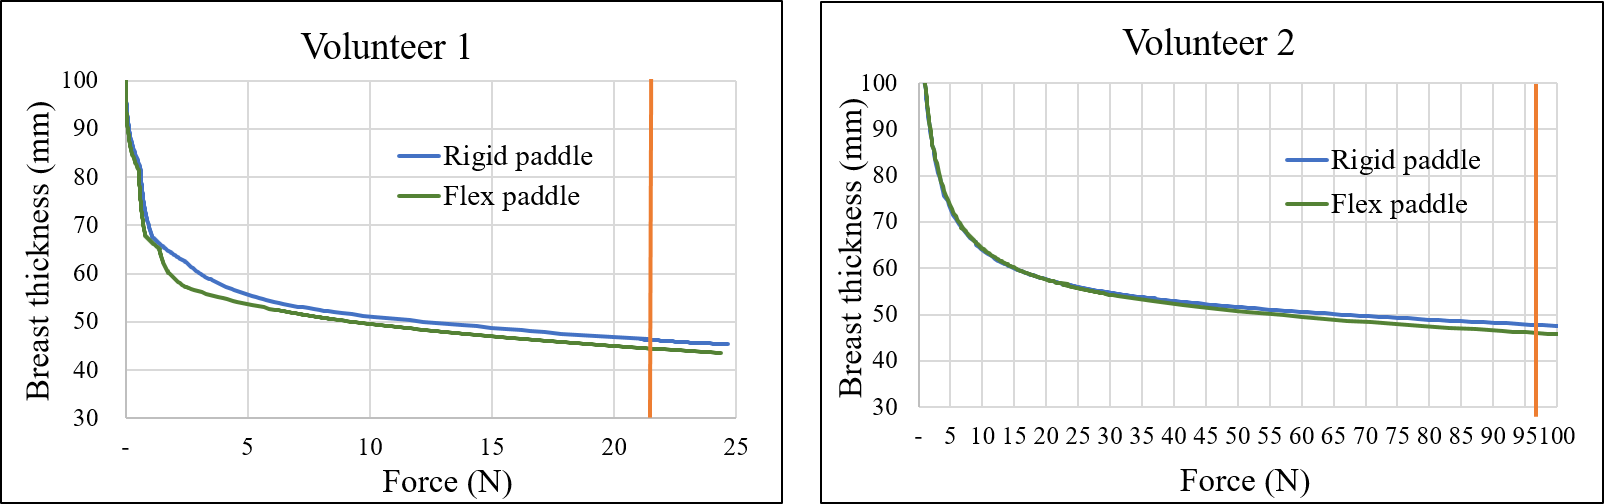
\includegraphics[width=1\textwidth,keepaspectratio]{figures/forceThicknessResults.png} 
\caption{Resulting breast flattening curve as function of the compression force with Gent constitutive model. }\label{fig:forceThicknessResults}
\end{figure}
    
 One can see that the compression force range is comparable with the one measured during mammography. Moreover, the curve behavior is similar with the one given by Groot et al \citep{de_pain_2015}, with an asymptotic behavior at the end of breast compression.
 
 In this section, it was assumed that introducing a Gent strain energy function will have a non-significant impact on breast mechanics under gravity loading since the Neo-Hookean and the Gent models have similar behaviors for small deformations. Therefore we can consider that the previous optimization process performed on the breast volume of the first volunteer remains valid. 
 
 \subsection{ Gent model and breast mechanics under gravity loading}
 
 When looking back to the Gent function properties, an appropriate  $J_m$ parameter was defined as following. The $J_m$ value has to be small enough in order to obtain an appropriate compression force. In the same time, it has to be high enough in order to preserve the fidelity of the model to the gravity loading deformations computed with a Neo-Hookean material.
 
 In Chapter \ref{chapter:myBioMecaModel}, the biomechanical breast model corresponding to the first volunteer was evaluated for Neo-Hookean material models. The worst estimate was found in supine tilted configuration due to the tissues oversliding on the lateral direction (maximal distance of $26.03 \ mm$). Introducing Gent tissues model should not impact the breast deformation under gravity loading. However, when looking at the supine tilted configuration simulated with Neo-Hookean material, large deformations were observed at the fascia and skin surfaces. Figure \ref{fig:strain_range_neo} shows the strain rates in supine, prone and supine tilted configurations obtained with Neo-Hookean material models. The strain rates over the skin and fascia surfaces in supine tilted configuration were twice larger than the ones observed in supine and prone configurations. Therefore, considering the Gent model in the multi-loading gravity simulations may improve the supine tilted estimate by reducing the fascia and skin deformations under large strains. 


\begin{figure}[!h]
\centering
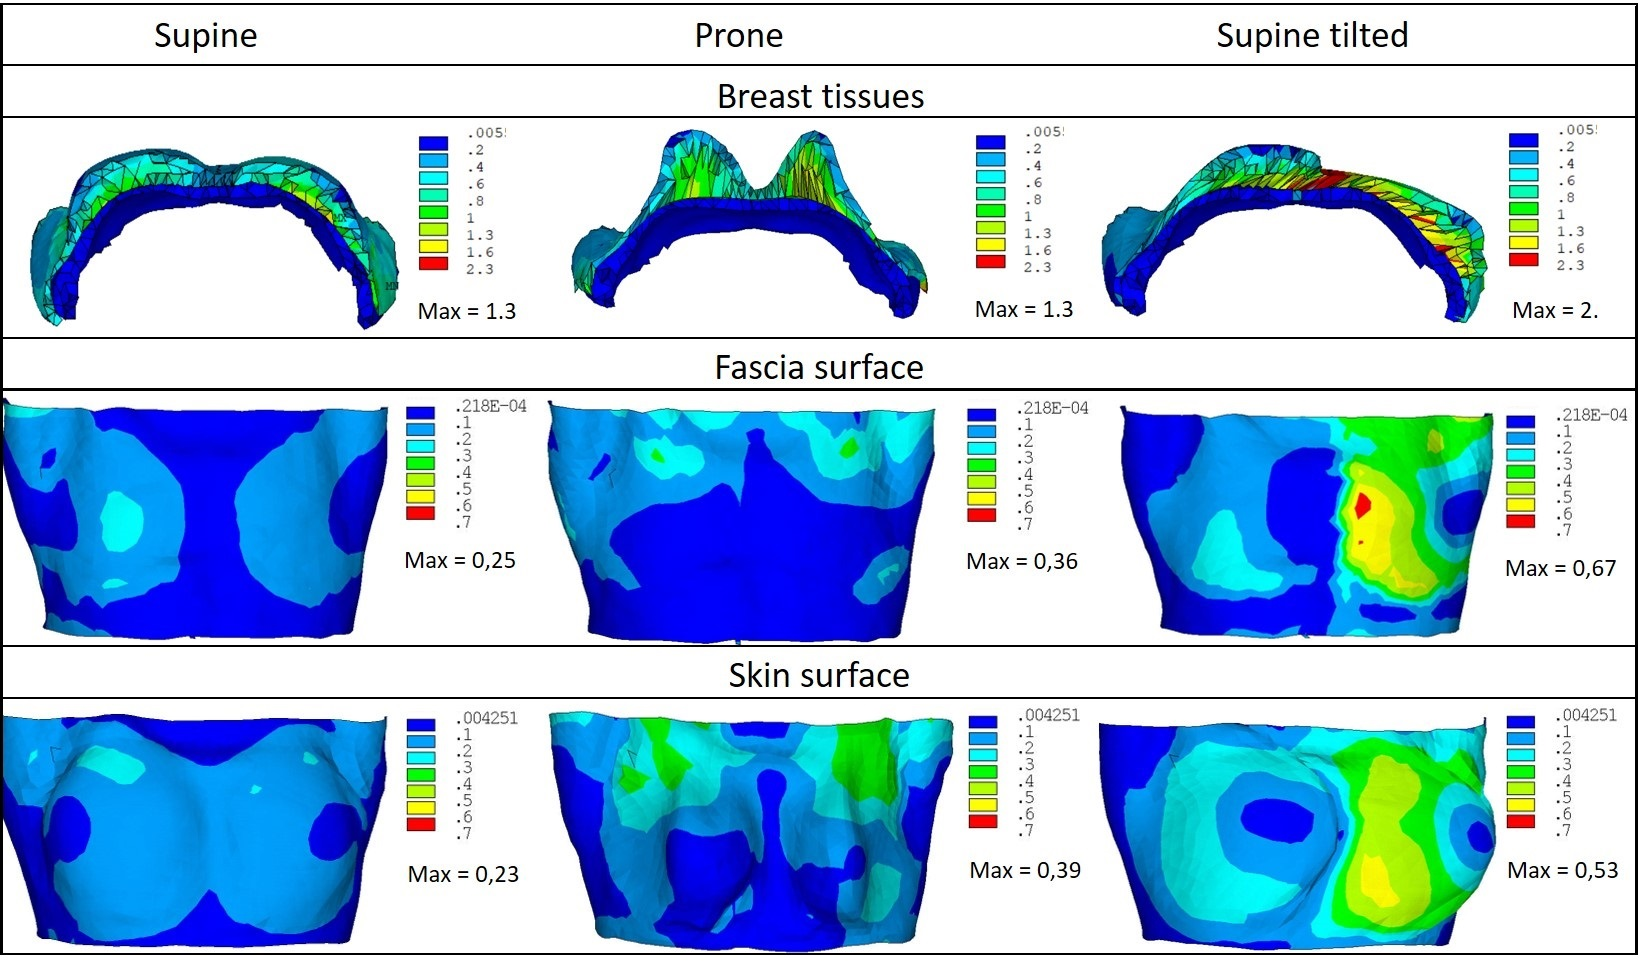
\includegraphics[width=\textwidth,keepaspectratio]{figures/strain_range_neo.jpg} 
\caption{Strain range distribution when using a Neo-Hookean material model. }\label{fig:strain_range_neo}
\end{figure}
 

\begin{figure}[!h]
\centering
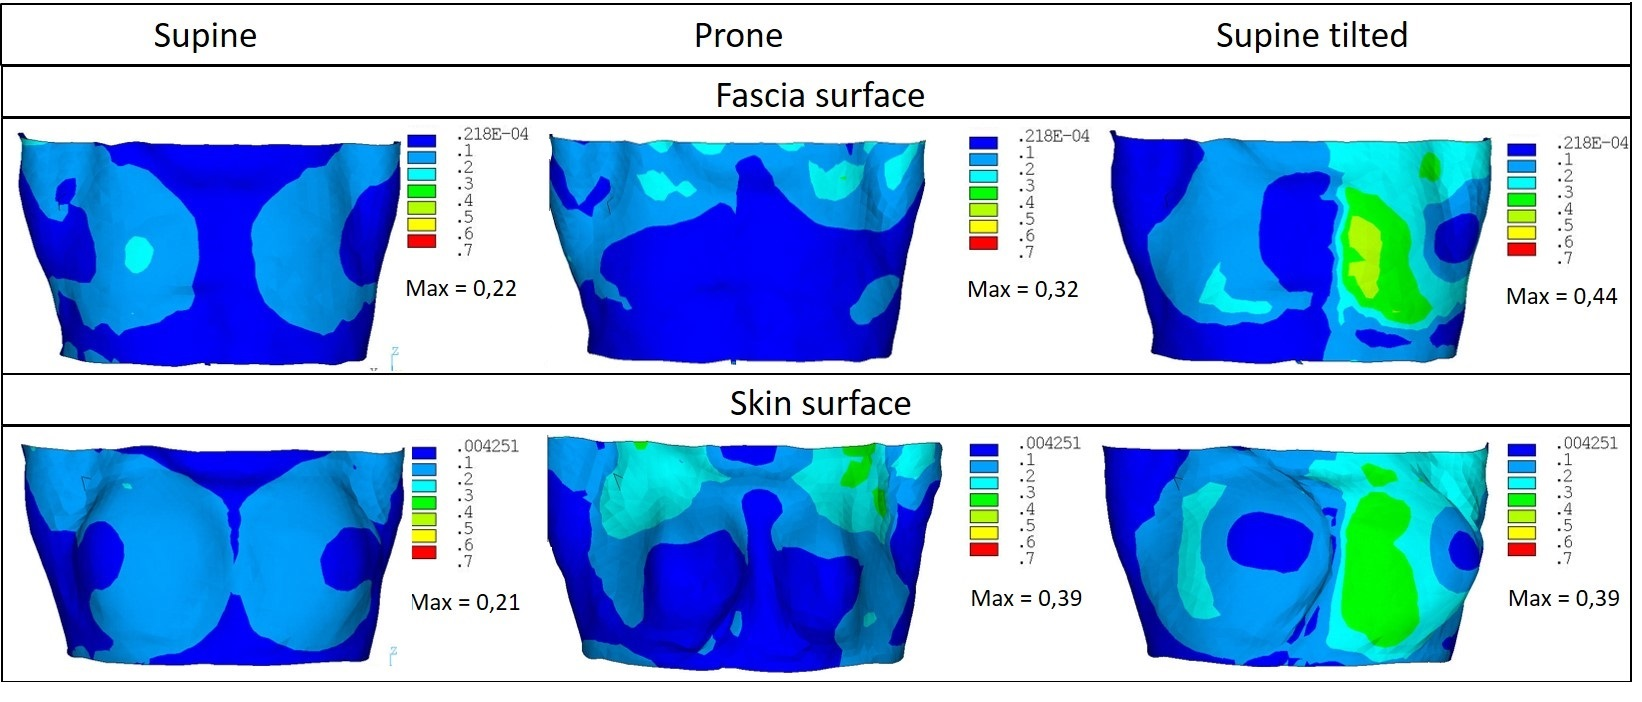
\includegraphics[width=\textwidth,keepaspectratio]{figures/strain_range_gent.jpg} 
\caption{Strain range distribution when using a Gent material model. }\label{fig:strain_range_gent}
\end{figure}

 Several simulations were performed considering $J_m = 1$, as identified during the compression simulations. However this value seems to constrain too much the tissues deformation in prone and supine configurations. It will be shown that the compression force is highly dependent on the paddle positioning with respect to the chest wall (Section \ref{subsection:breastpositioning}). For an accurate estimation of the parameter $J_m$, more data is needed concerning the paddle position during compression. In our study, the paddle position with respect to the chest wall was not available. Therefore, the estimated $J_m$ value is only an approximation and does not characterize completely the subject breast mechanics.    
 
When the multi-loading gravity simulations were performed using a Gent model with $J_m=2$, better estimates were obtained. In this respect, to show the impact of using a Gent model within multy-loading gravity simulations, the parameter $J_m$ of all involved tissues was set to 2. Figure \ref{fig:strain_range_gent} shows the corresponding strain range distributions over the skin and fascia surfaces.  The maximal strain does not change significantly in supine and prone configurations ( less than $10\%$ of difference). On the other hand, important changes were observed over the left breast in supine tilted configuration. The maximal strain range decreased by about $30\%$ over the fascia surface and by about $26 \ \%$ over the skin surface. As previously described, these tissues provide the breast support, accordingly,  the lateral displacement of the left breast was reduced.

 The estimates of breast external geometry in the three configurations computed using the Gent material models are presented in Figure \ref{fig:modelevaluation_gent}. One may see that the breast deformations in supine and prone configurations remain on the same range of precision. The Hausdorff distance being increased by only $0.46 \ mm$ and $0.6\ mm$ respectively (maximal distance by $0.17\ mm$ and $0.93 \ mm$ respectively). Contrariwise, the sliding of the left breast was significantly reduced. Even if the Hausdorff distance was reduced by only $1 \ mm $ ($5.15 \ mm$ with Gent models versus $6.14 \ $ with Neo-Hookean models), a significant decrease of $10 \ mm$ in maximal distance  was observed. Moreover, smaller deformations imply also better solution convergence. 
   

\begin{figure}[!h]
\centering
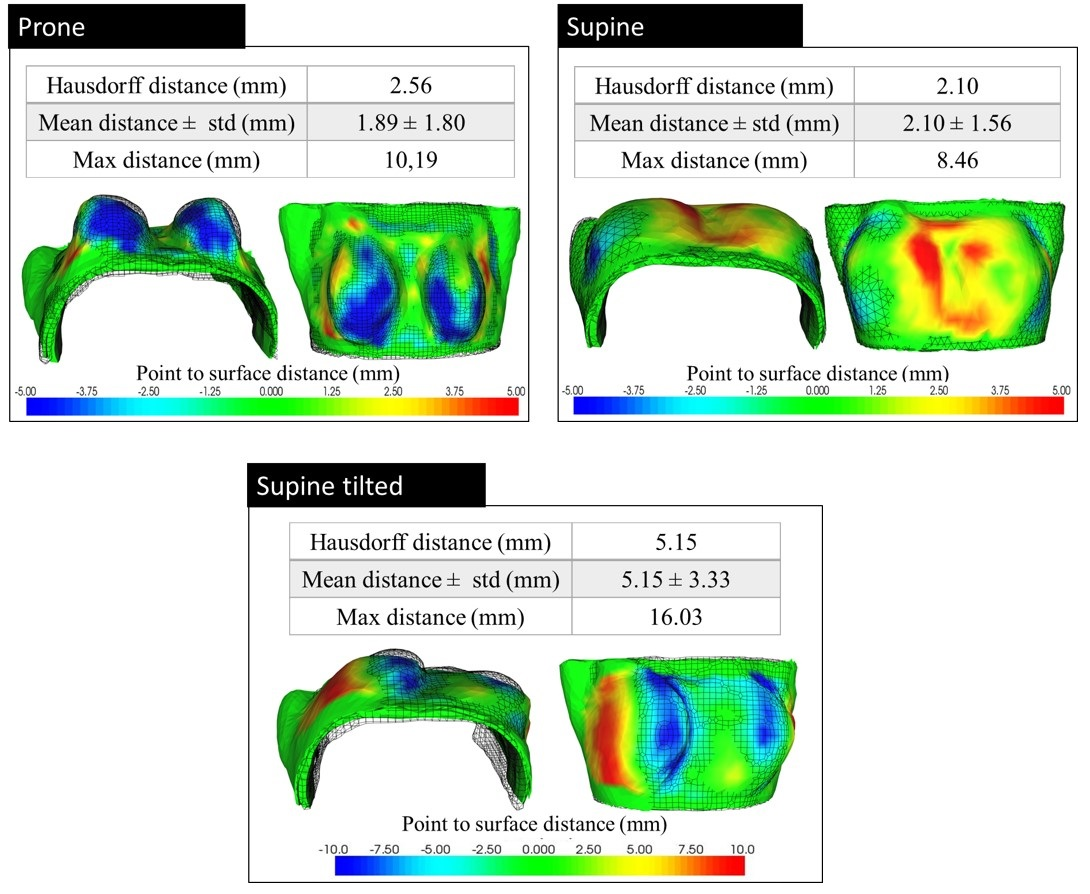
\includegraphics[width=\textwidth,keepaspectratio]{figures/modelevaluation_gent.jpg} 
\caption{Difference between estimated and measured breast surfaces, in supine, prone and supine tilted configurations obtained with a Gent material model. }\label{fig:modelevaluation_gent}
\end{figure}

Using the Gent model improved the overall performance of the breast biomechanical model. However, different values of  parameter $J_m$ were used to simulate breast deformations under compression and under gravity loading. A more detailed study is needed to find appropriate constitutive parameters characterizing a wider panel of breast deformations.  

 In this chapter we assumed a constant value of $J_m$ for all involved hyperelastic material models, while their mechanical response under large stresses are different. A variable $J_m$ parameter within tissues types may improve model accuracy.  On the other hand, it also implies an optimization process with more constitutive parameters. An optimization process with a higher number of variables is also more expensive in terms of data and time resources. 
 
 For the breast compression simulations presented below the parameter $J_m$ for the first volunteer was set to 1. This assumption satisfies the thickness-force  relation obtained during the mammography exam.

\section{Simulation of digital images }
Once the compression simulations were performed, the compressed breast geometry was extracted and used to create numerical object defined by the means of a surface meshes, also named numerical phantoms. These objects were used as input for the CatSim environment able to simulate a digital mammography  acquisition \citep{de_low_2014,de_catsim_2007}. The simulated images were used to assess the image quality as function of the compression paddle design.

\subsection{Physical characteristics}
The X-ray projections of phantom objects were simulated using a GE Senographe Pristina system topology (Figure \ref{fig:systemgeometry}). The focal spot was modeled as a point source. A $24\ keV$ mono-energetic X-ray beam was considered.  This beam quality is similar to the effective X-ray energy of a $34\ kVp$ Rh/Ag target/filter spectrum filtered by a $46\ mm$ compressed breast. Spreading of the light photons in the CsI scintillator of the detector was modeled by filtering the detected X-ray beam by an empirically assessed modulation transfer function of the cesium iodide (CsI) scintillator. X-ray scatter from the test object and other system components were not included in the simulation. Only quantum noise, modeled by a Poisson random distribution, was considered as noise source. The simulated X-ray flux was tuned to match the average signal intensity ($\langle SI \rangle$) and signal-to-noise ratio (SNR) measured in real images of a $46\ mm$ thick, $20\%$ fibroglandular equivalent phantom acquired with the automatic exposure control. To do so, a calibration was performed on a real Senographe Pristina mammography unit.


\begin{figure}[!h]
\centering
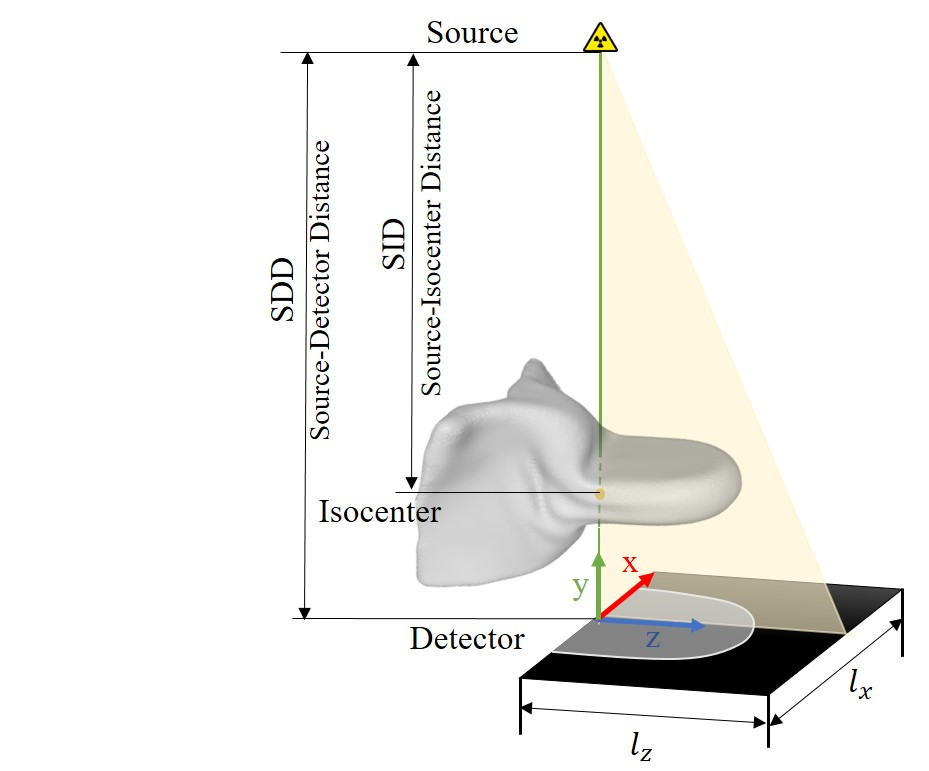
\includegraphics[width=0.65\textwidth,keepaspectratio]{figures/systemgeometry.jpg} 
\caption{A schematic illustration of the simulated GE Senographe Pristina $^{TM}$ mammography unit.}
\label{fig:systemgeometry}
\end{figure}
%SDD = 660mm, SID = 636.76 

\subsection{Breast phantom objects}

The phantoms were created by first extracting the compressed breast external shape. Then, a set of virtual microcalcifications ($\mu calc$) was inserted into each compressed breast volume. The smallest breast volume contains 21 microcalcifications arranged in a matrix of 7 rows and 3 columns (Figure \ref{fig:microcalcifications}.a). The largest breast volume contains 56 microcalcifications arranged in a matrix of 7 rows and 8 columns. The matrix of $\mu calc$ was parallel with the entrance surface of the image receptor and was positioned at the breast mid thickness (Figure \ref{fig:microcalcifications}.b). The distance between two consecutive columns or rows was equal to $10\ mm$. The anatomical background was assumed to be a uniform breast-equivalent material composed of glandular/adipose tissue with a $20/80$ ratio. Two simulations were performed for each compression considering microcalcifications of $0.2\ mm$ and $0.3\ mm$ in diameter.

\begin{figure}[!h]
\centering
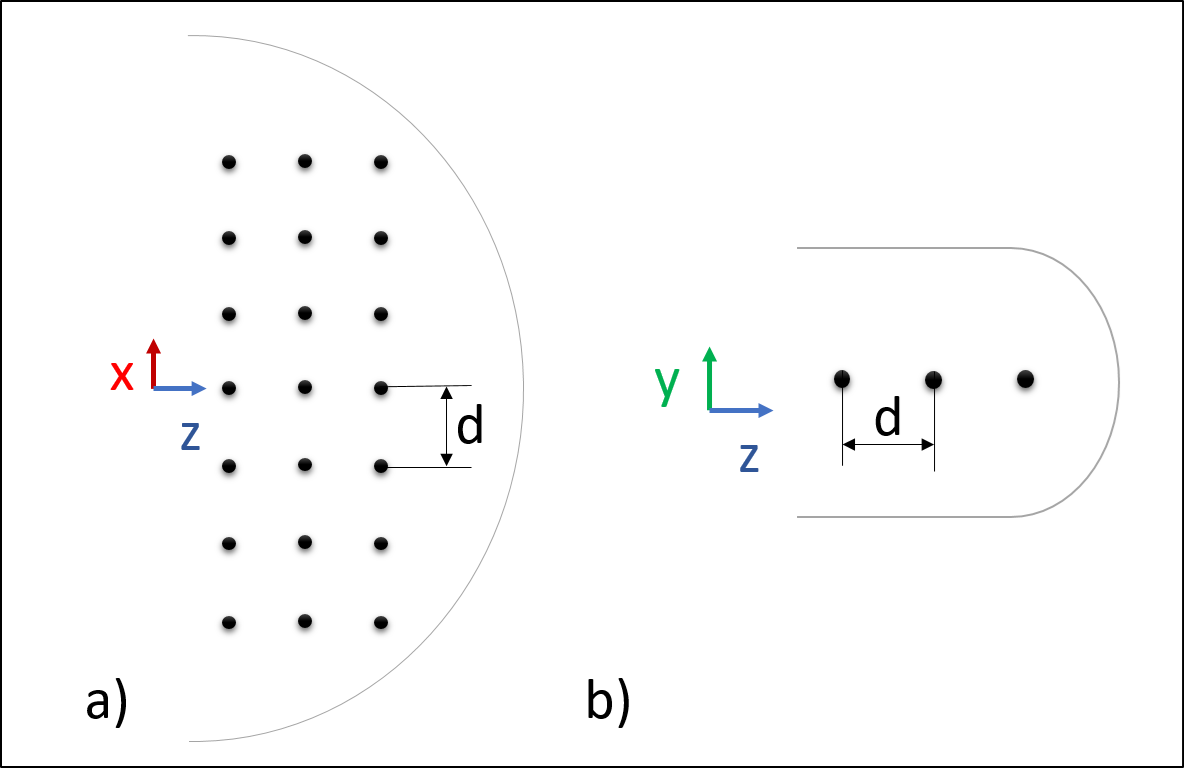
\includegraphics[width=0.5\textwidth,keepaspectratio]{figures/microcalcifications.png} 
\caption{Microcalcification distribution over the smallest breast volume $(d=10mm)$: a) axial view, b) sagittal view.}\label{fig:microcalcifications}
\end{figure}


Microcalcifications were simulated as round-shaped surface mesh. To add irregularities, initially spherical objects were randomly deformed. Their X-ray attenuation properties were chosen to correspond with the attenuation of aluminium (Al) at $24 \ keV$, their volumetric mass density correspond to $60\%$ of the Al density (i.e. $1.63\ \frac{kg}{m^3}$).  The choice of $24\ keV$ corresponds to the photon energy of the X-ray source used in our study. 


\section{Compression quality metrics}\label{section:compressionqualitymetrics}

The measures used to quantify the three criteria characterizing the quality of breast compression (patient comfort, image quality and average glandular dose) are described in the following section.  

\subsection{Patient comfort}

Today, pain estimation and quantification still remain an open question. The perceived pain during mammography, or its interpretation, may depend on the social status, pain history or psychological condition of the patient. But it also depends on physical parameters such as compression force, amount of strain or pressure at skin surface. In clinical studies, the patient comfort is assessed using pain scales. The repeatability of such methods is questionable, because they are based on the patient own interpretation and expertise. More quantitative measures such as pupil dilatation or heart beat rate are interesting in assessing the patient comfort; however they may indicate not only the pain but also the fear of pain.        

In this work, only physical pain associated with tissues deformations was considered. In this scope, the maximal strain and stress intensities as well as the maximal pressure intensity at the contact surface were chosen as pain quantifiers. Their distribution over the breast volume were obtained from FE simulations of breast compression and were analysed in order to compare the patient experience between two distinct compression systems. 

\subsection{Image quality }\label{section:averagegalndulardose}
 To assess image quality, the signal-difference-to-noise ratio (SDNR\nomenclature{SDNR}{Signal Difference to Noise Ratio})  and the signal-to-noise ratio (SNR\nomenclature{SNR}{Signal to Noise Ratio})  were measured in the raw simulated images. To this end, squared ROIs of  $1cm \times 1cm$ were defined centered on the $\mu calcs$ position. The pixels inside of each ROI were divided into two sets. Pixels located  at the ROI's center within a radius equal to the radius of the $\mu calcs$  represent the $\mu calcs$ attenuated signal intensity ($SI_{\mu calc}$). Pixels located within the ROI but outside the $\mu calc$ radius represent the background signal intensity ($SI_{back}$). The two sets were used to compute the average detected signal per $\mu calcs$ pixel ($\langle SI_{\mu calc}\rangle$), the average detected signal per background pixel  ($\langle SI_{back}\rangle$) and the standard deviation in the background signal intensity $\sigma_{back}$:
 \begin{align}
 \langle SI_{\mu calc}\rangle& = \frac{1}{\vert SI_{\mu calc}\vert} \sum_{p_i \in SI_{\mu calc}}p_i \\
  \langle SI_{back}\rangle &= \frac{1}{\vert SI_{back}\vert} \sum_{p_i \in SI_{back}}p_i\\
  \sigma_{back} &= \sqrt{\frac{1}{\vert SI_{back}\vert} \sum_{p_i \in SI_{back}} (p_i- \langle SI_{back}\rangle)^2}
  \end{align}
Where $\vert\cdot\vert$  is the number of pixels in the respective set.

  The SDNR per pixel of the inserted microcalcifications is defined as follows
 \begin{equation}
 SDNR = \frac{\langle SI_{back}\rangle - \langle SI_{\mu calc}\rangle}{\sigma_{back}},
\end{equation}

 
The SNR per background pixel was defined as follows  
 \begin{equation}
 SNR = \frac{\langle SI_{back}\rangle}{\sigma_{back}}.
\end{equation}



\subsection{Average glandular dose}
The estimation of the dose delivered to the glandular tissue remains an essential component of quality control in X-ray mammography. We derived the average glandular dose (AGD) using the approach proposed by Dance D. \citep{dance_additional_2000} regardless the paddle type. The method uses conversion factors to relate measurements of the incident air kerma $K$ at the upper surface of the breast to the AGD. 

\begin{equation}
AGD = K g c s
\end{equation}

where $g$ is the factor allowing to convert air kerma to AGD considering a breast with 50\% glandularity, $c$ addresses any difference in breast composition from this 50\% glandularity and s accounts for the X-ray spectrum under consideration. Dance et a. used Monte-Carlo simulation to estimate these factors by modeling the compressed breast as a semi-circular cross section cylinder. The $s$-factor for the recently introduced Rh/Ag target/filter spectrum was provided to us by D. Dance and has not been published yet.

The considered cross section cylinder has a uniform thickness, meanwhile the compressed  breast thickness varies due to paddle elasticity (SRP) and paddle flexibility (SFP). Therefore, in a clinical framework, the breast thickness is adjusted by applying an offset characterizing the paddle deflection during compression.      

For the rigid paddle model, as paddle elasticity was neglected, the AGD was computed assuming the breast thickness is equal to the distance between the image receptor and the paddle itself. Regarding the flex paddle, the breast thickness decreases quasi-linearly from the chest wall to the nipple. Thus, breast thickness was computed as the mean of the maximal and minimal distance over the breast contact area.

\section{Results}\label{section:breastcompressionevaluation}
Two studies were performed using the previously defined components for modeling the breast compression and simulating digital mammography. First, the results of a comparative study between flex and rigid paddles is presented with the effects on image quality, AGD and patient comfort. Then, the impact of paddle positioning on breast mechanics is analysed.   
\subsection{Compression quality for rigid and flex paddles}

To compare the breast compression quality when using a standard rigid paddle against a standard flex paddle, the rigid and flex paddle models were used. The right breasts of the two volunteers were first compressed until the target breast thickness measured during mammography was obtained (Table \ref{tab:forceandthichnessdata}). Then, the breast phantoms with $\mu calc $ were imported into CatSim environment and mammography images were simulated. The compression quality was measured in terms of image quality, AGD and patient comfort.

The resulting average breast thickness after compression varies by less than $2mm$ between rigid and flex paddles for both volunteers (Table \ref{fig:table_compression_results}). Accordingly, small AGD differences were found and namely dose reductions of $2.6 \%$ for the smaller breast and $4.2\%$ for the larger breast were observed in favor of the flex paddle.

\begin{figure}[!h]x-ray
\centering
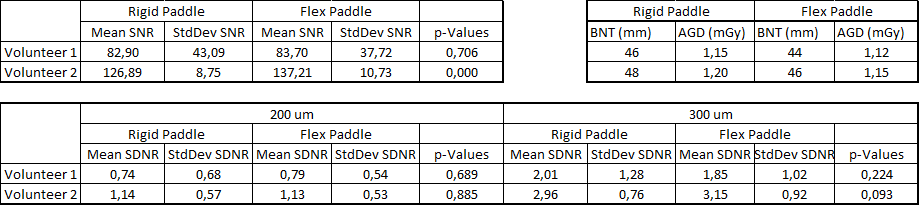
\includegraphics[width=\textwidth,keepaspectratio]{figures/table_compression_results.png} 
\caption{Breast nominal thickness (BNT), average glandular dose (AGD), signal-to-noise-ratio (SNR) and signal-difference-to-noise (SDNR) for both volunteers and both compression paddle types}\label{fig:table_compression_results}
\end{figure}

The SNR and SDNR have been estimated and compared between flex and rigid paddles. When using a flex paddle instead of a rigid paddle on the largest breast (volunteer 2), we observed a statistically significant higher SNR. We did not observe statistically significant differences on SDNR for both $200\mu m$ and $300\mu m$ microcalcifications, when using rigid or flex paddle. Therefore, despite a breast thickness varying linearly from chest wall to nipple when the flex compression paddle is used, the image quality is preserved or improved compared to the image quality obtained with the rigid compression paddle.

In a clinical study, Broeders et al. \citep{broeders_comparison_2015} have also compared the image quality and patient comfort between the standard rigid and flex paddles. According to the authors, the standard flex paddle performed slightly better image quality in the projected breast area, however it moved breast tissue from the image area at chest wall side. According to our compression simulation, for the small breast volume, no difference in tissues lateral displacement was observed. On the other hand, for the larger breast, using the flex paddle indeed increased the tissues displacement toward the chest wall side, but not by more than $4 \ mm$ (Figure \ref{fig:rigid_flex_y_displacement}).  

\begin{figure}[!h]
\centering
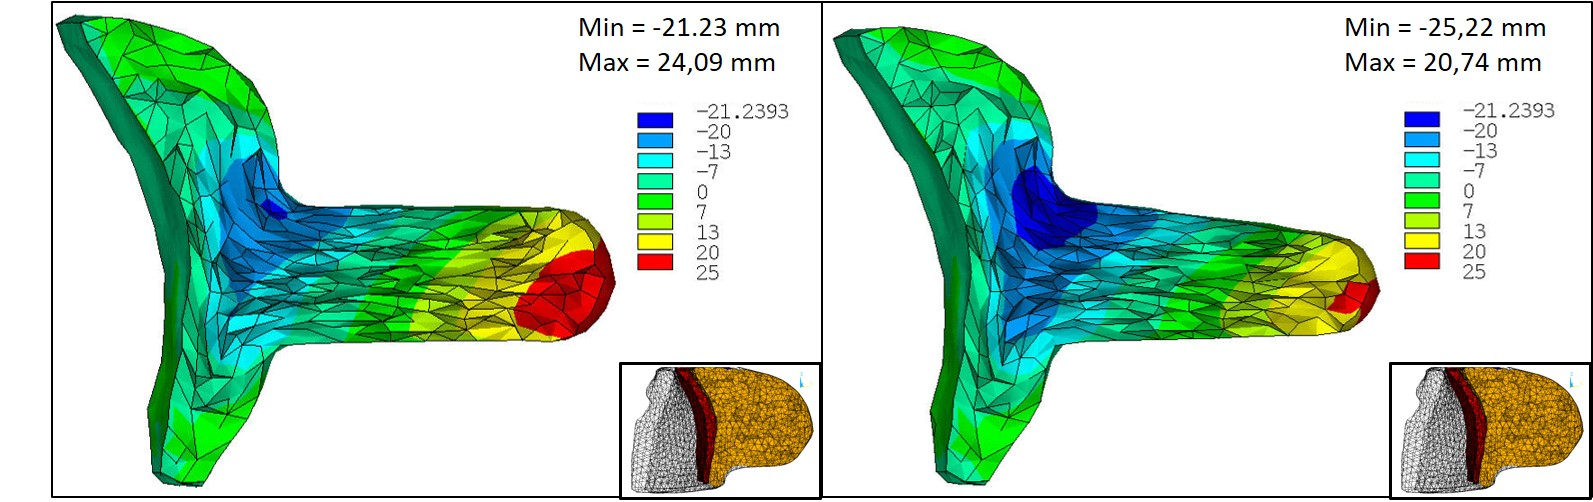
\includegraphics[width=1\textwidth,keepaspectratio]{figures/rigid_flex_y_displacement.jpg} 
\caption{Node displacements on the direction parallel to the paddle (Oy axis). Left hand side - rigid paddle, right hand side flex paddle.}\label{fig:rigid_flex_y_displacement}
\end{figure}

To assess the patient comfort during compression, the resulting internal stress and strain distributions, as well as the contact pressure maps were derived. These data were collected at compressive forces of 22 $N$ for the first volunteer (Figure \ref{fig:subject1_compressionResults}) and 95 $N$ for the second one (Figure \ref{fig:subject2_compressionResults}).

\begin{figure}[h!]
\centering
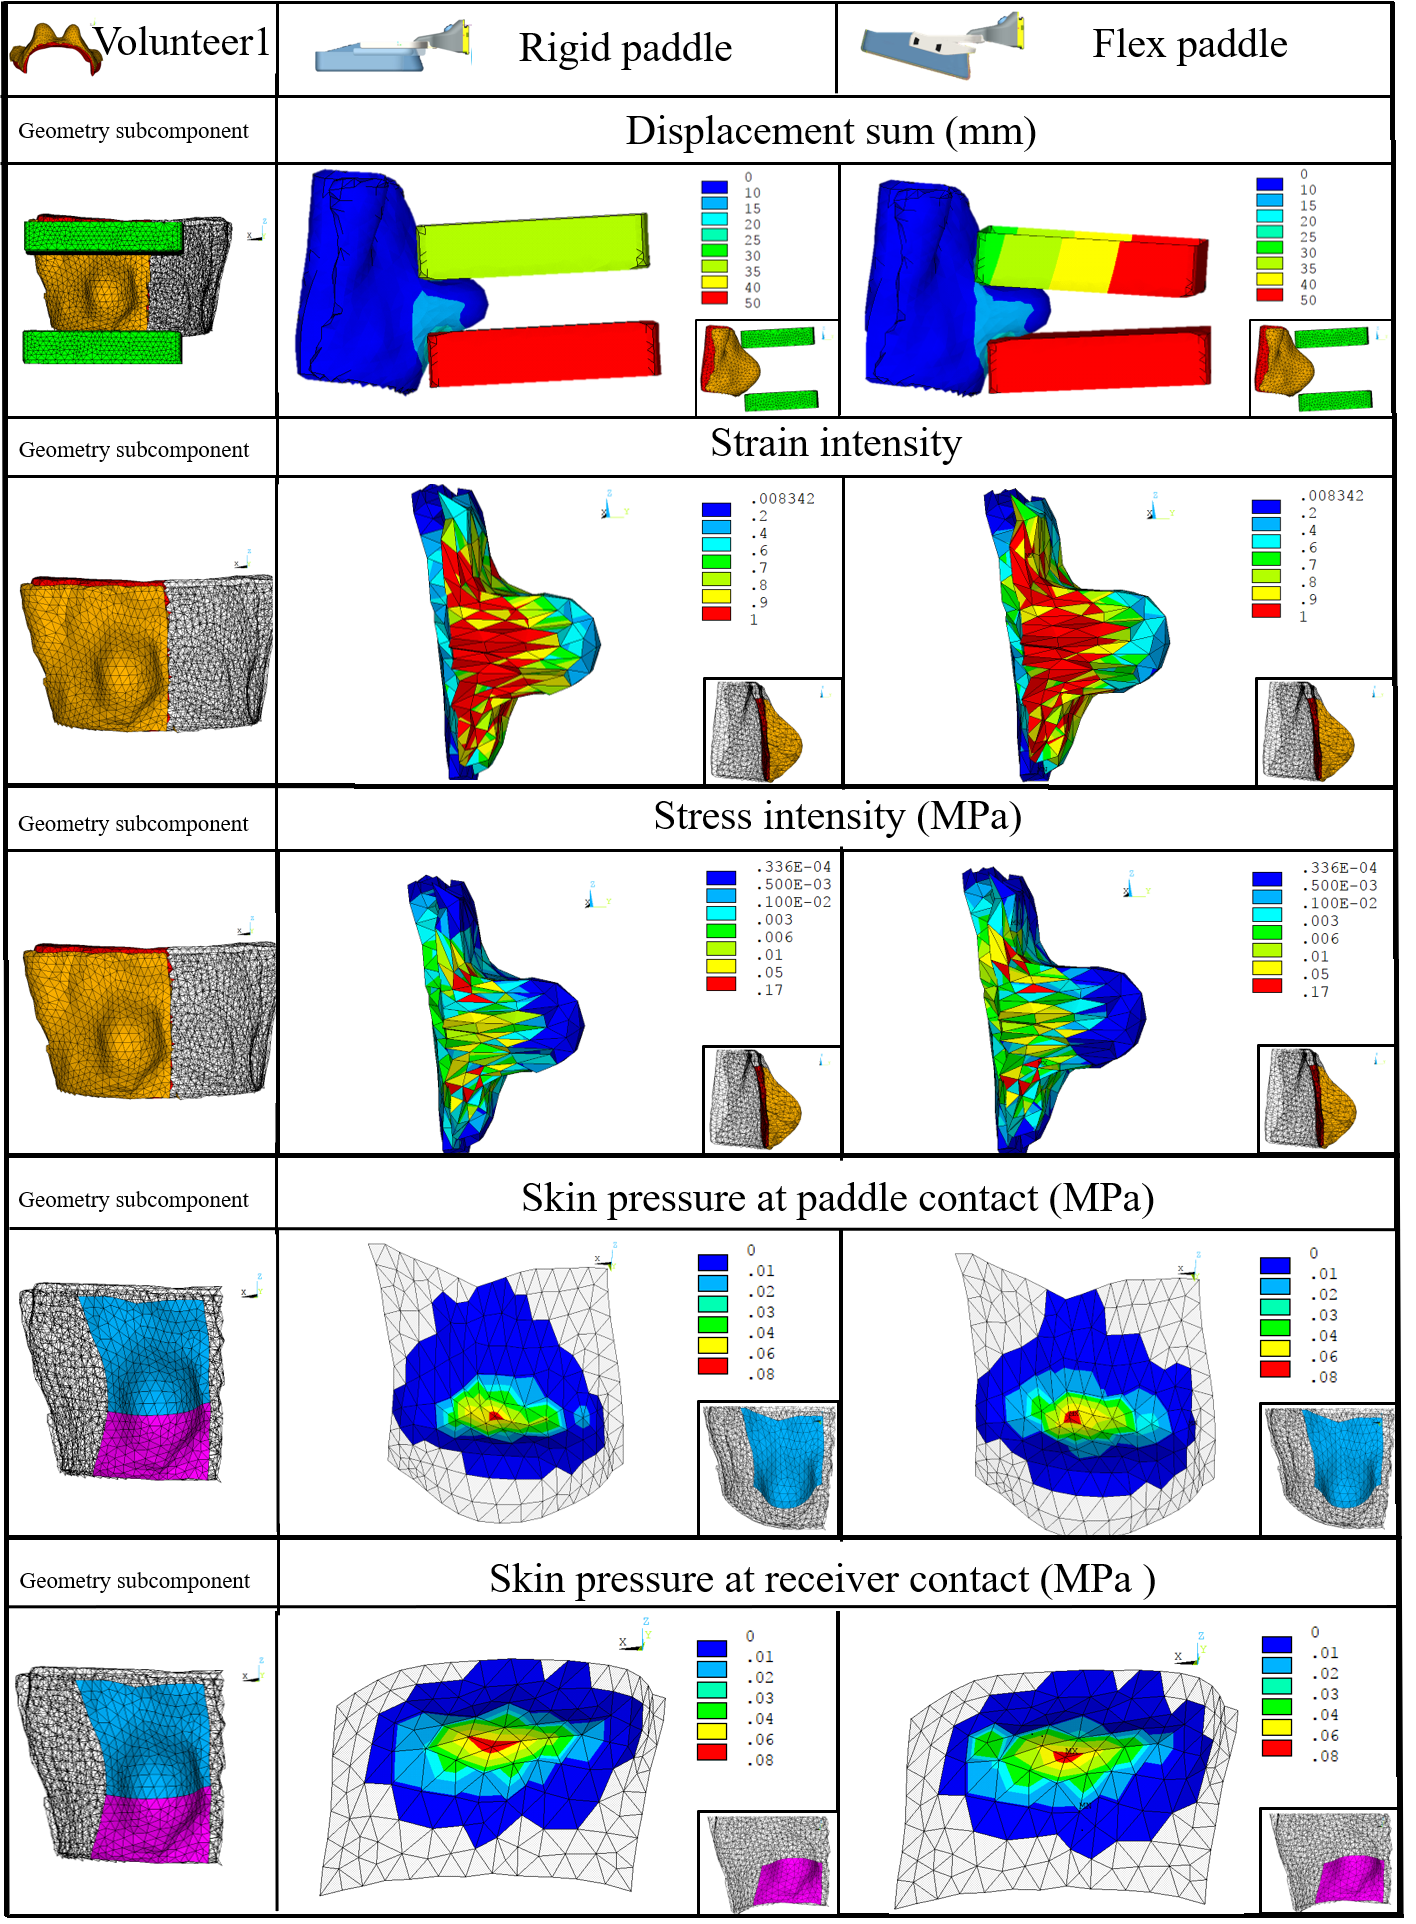
\includegraphics[width=0.9\textwidth,keepaspectratio]{figures/subject1_compressionResults.png} 
\caption{Stress, strain and contact pressure distribution for the first volunteer}\label{fig:subject1_compressionResults}
\end{figure}

\begin{figure}[h!]
\centering
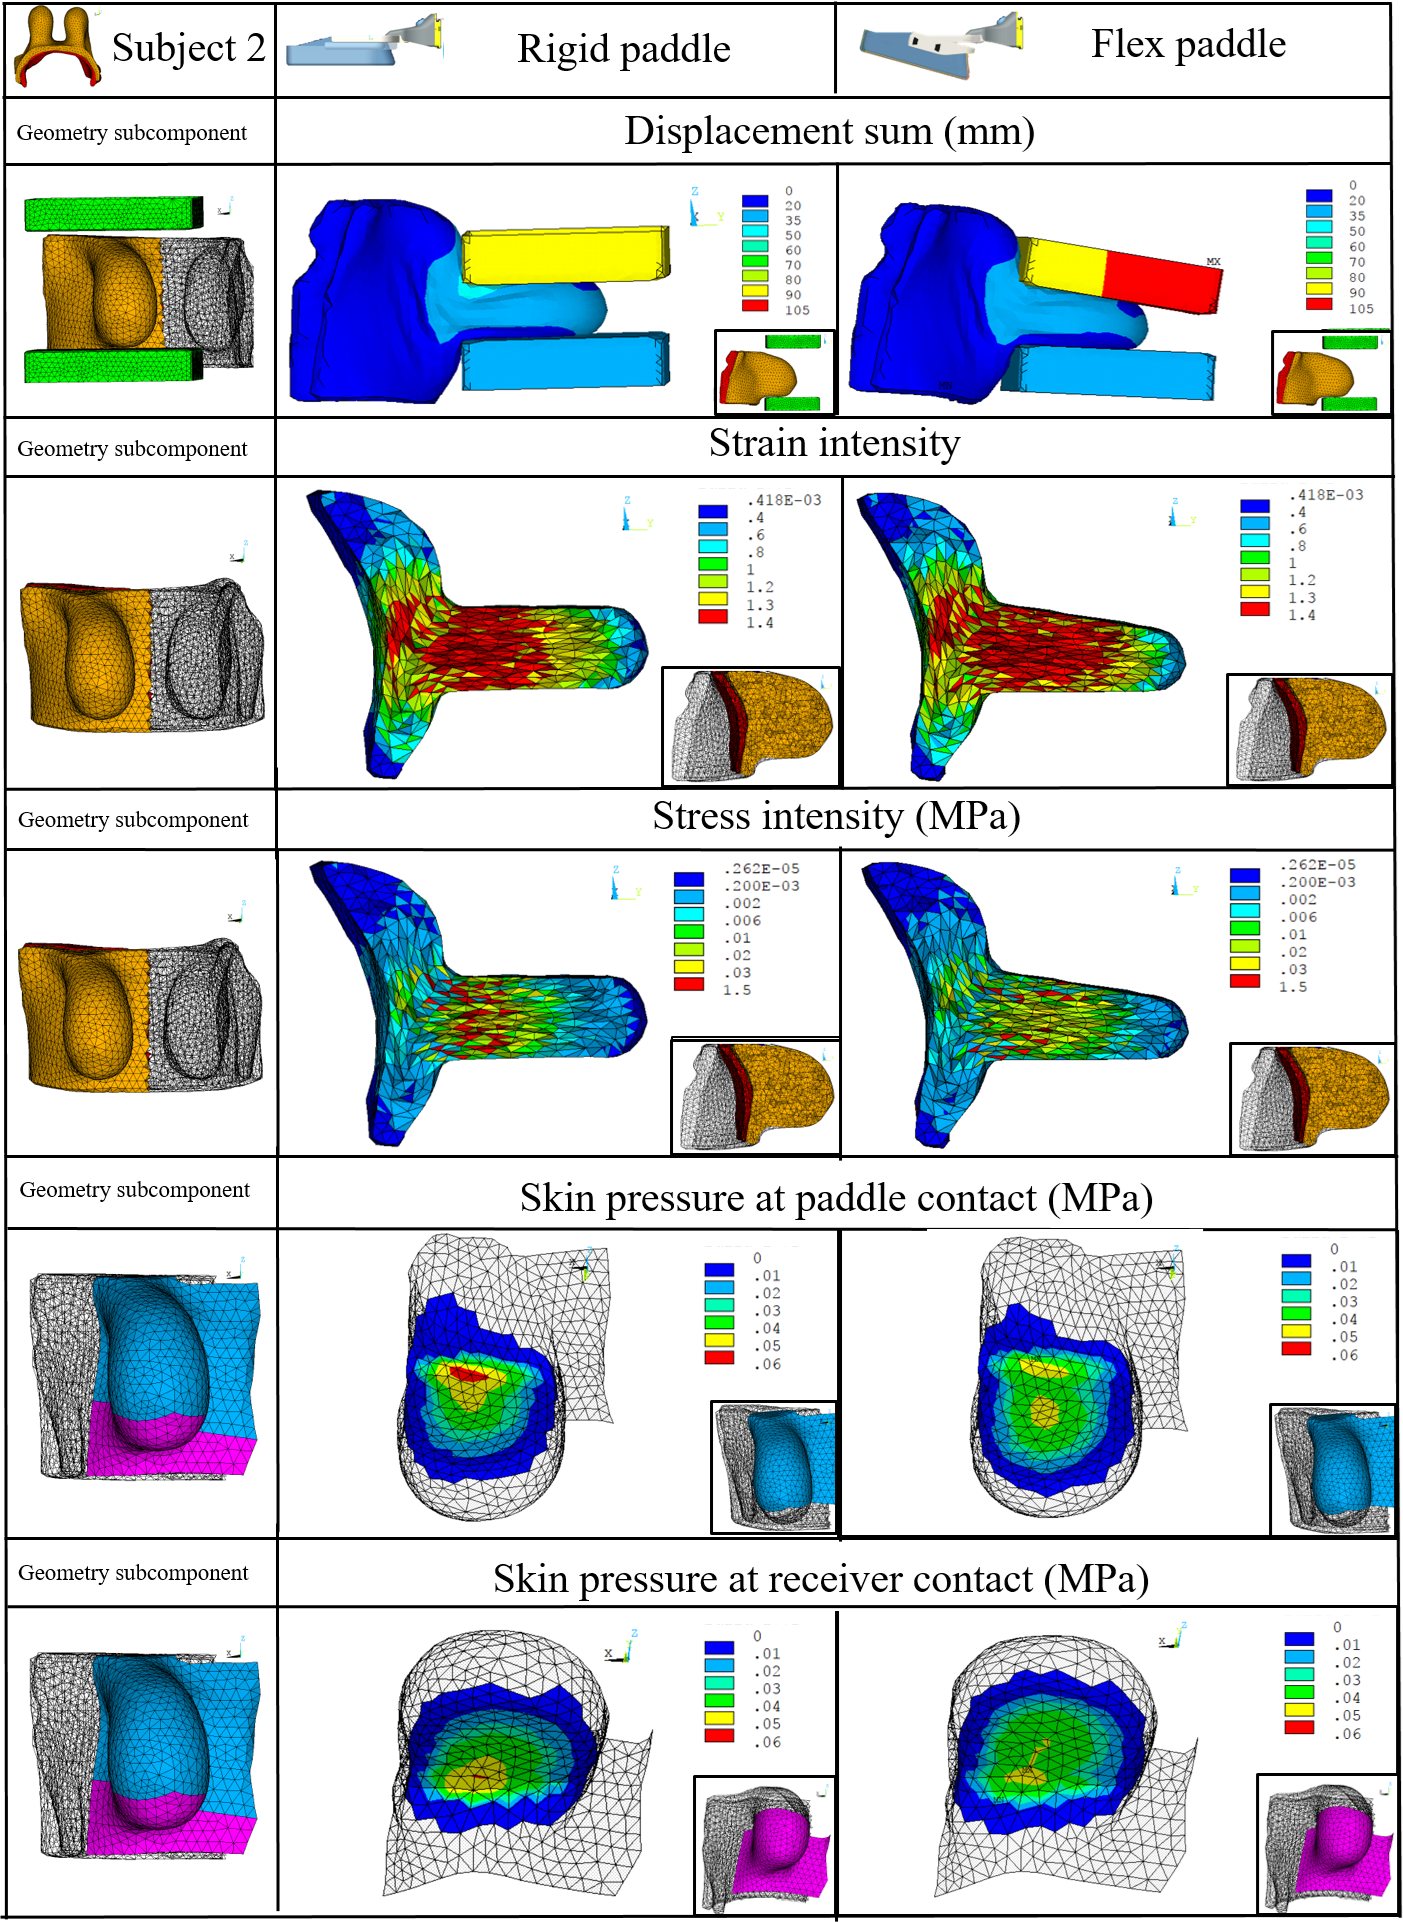
\includegraphics[width=0.9\textwidth,keepaspectratio]{figures/subject2_compressionResults.png} 
\caption{Stress, strain and contact pressure distribution for the second volunteer}\label{fig:subject2_compressionResults}
\end{figure}


Regarding the smallest breast volume (Figure \ref{fig:subject1_compressionResults}), there is no significant difference between FPM and RPM in pressure distribution over the skin surface or in internal stress/strain intensity distributions. For both compression paddles, high pressure at the skin surface is concentrated in the juxtathoracic region with a maximum pressure of 77.7 $kPa$. In addition, the FE simulations confirm that in small breasts the paddle tilt is too small to impact the tissues compression in the middle part of the breast. FPM applied on larger breast volumes (Figure \ref{fig:subject2_compressionResults}) results in significantly lower intensities of pressure at the skin surface in contact with the compression paddle, with a maximal pressure of 37 $kPa$, compared to 56 $kPa$ when using RPM. No significant difference in the measured maximal intensities of strain and stress was observed, however strain and stress distribution patterns are different. When the breast is compressed with a rigid paddle, maximal strain and stress are concentrated in the retromammary space and decrease considerably toward the nipple. When a flex paddle is used, stress and strain are more uniformly distributed over the breast volume with the highest values in the middle third of the breast.

The area pressure distribution patterns have already been demonstrated in the work by Dustler et al. \citep{dustler_breast_2012}. The authors have studied the pressure distribution patterns of 103 women undergoing breast compression with a rigid paddle at different compression levels. Four groups were differentiated: a) skin pressure widespread over the breast (29\%); b) skin pressure concentrated on the central part of the breast (8\%); c) skin pressure concentrated on the juxtathoracic region (16\%); d) skin pressure concentrated along a narrow zone at the juxtathoracic region (26\%).  The pressure distribution patterns observed for our first and second volunteers correspond to the group d) and a) respectively.


\clearpage
\subsection{Paddle positioning impact on compression mechanics}\label{subsection:breastpositioning}

A second study was performed in order to assess the paddle positioning impact on the compression force. The simulations were performed only on the right breast of the second volunteer. Indeed, the geometry of the first volunteer is too small and does not meet the necessary morphological criteria required by this study. 

Using the rigid paddle model to perform compressions with different paddle position in respect to the thoracic cage (thoracic cage to paddle distance TPD, Figure \ref{fig:elasticpaddle}) has generated large convergence problems. For example, when the paddle was positioned closer to the chest wall, the finite elements were distorted because of high contact pressure at the juxtathoracic are. Therefore, for further investigations, the elastic paddle model was used. This model is closer to the mechanical properties of the standard rigid paddle from a mammography unit.  In addition, material elasticity allows a slight paddle bending which seems to reduce elements' distortions. 

\begin{figure}[!h]
\centering
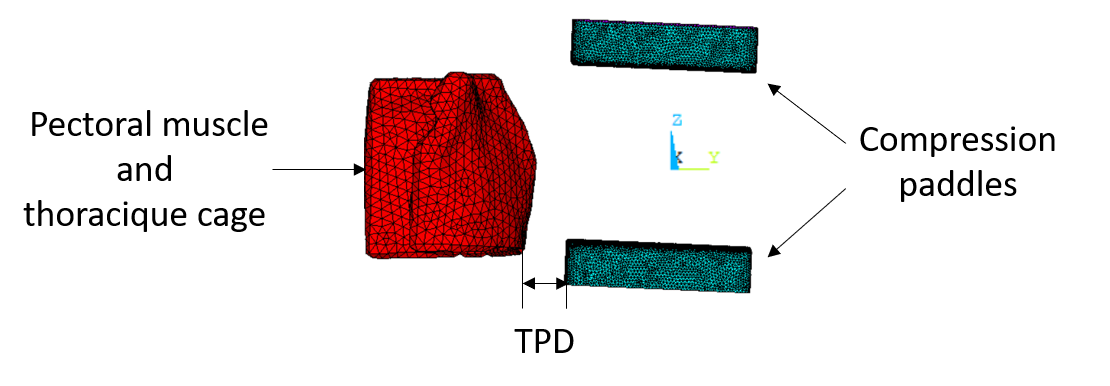
\includegraphics[width=0.8\textwidth,keepaspectratio]{figures/TPdistance.png} 
\caption{Thoracic cage to paddle distance (TPD).}\label{fig:elasticpaddle}
\end{figure}

 The breast was compressed until a minimal thickness of $50mm$ was reached. Then, the compression force as well as surface pressure at the contact with the compression paddle were compared. The compression force was computed as the product between the mean surface pressure and the contact area $\langle P_{contact}\rangle \ast  A_{contact}$.

Figure \ref{fig:elasticpaddle} shows the strain/stress as well as the pressure distributions over the contact area for three distinct distances between the thoracic cage and the paddle (TPD). The compression force varies considerably within paddle positions. A compression force of $59\ N$, $94\ N$ and $158\ N$ was obtained when the paddle was positioned at a distance from the chest wall of $48\  mm$, $40\  mm$ and $33\ mm$ respectively. Positioning the paddle with $15\ mm$ closer to the chest wall tripled the force intensity. 
 
\begin{figure}[!h]
\centering
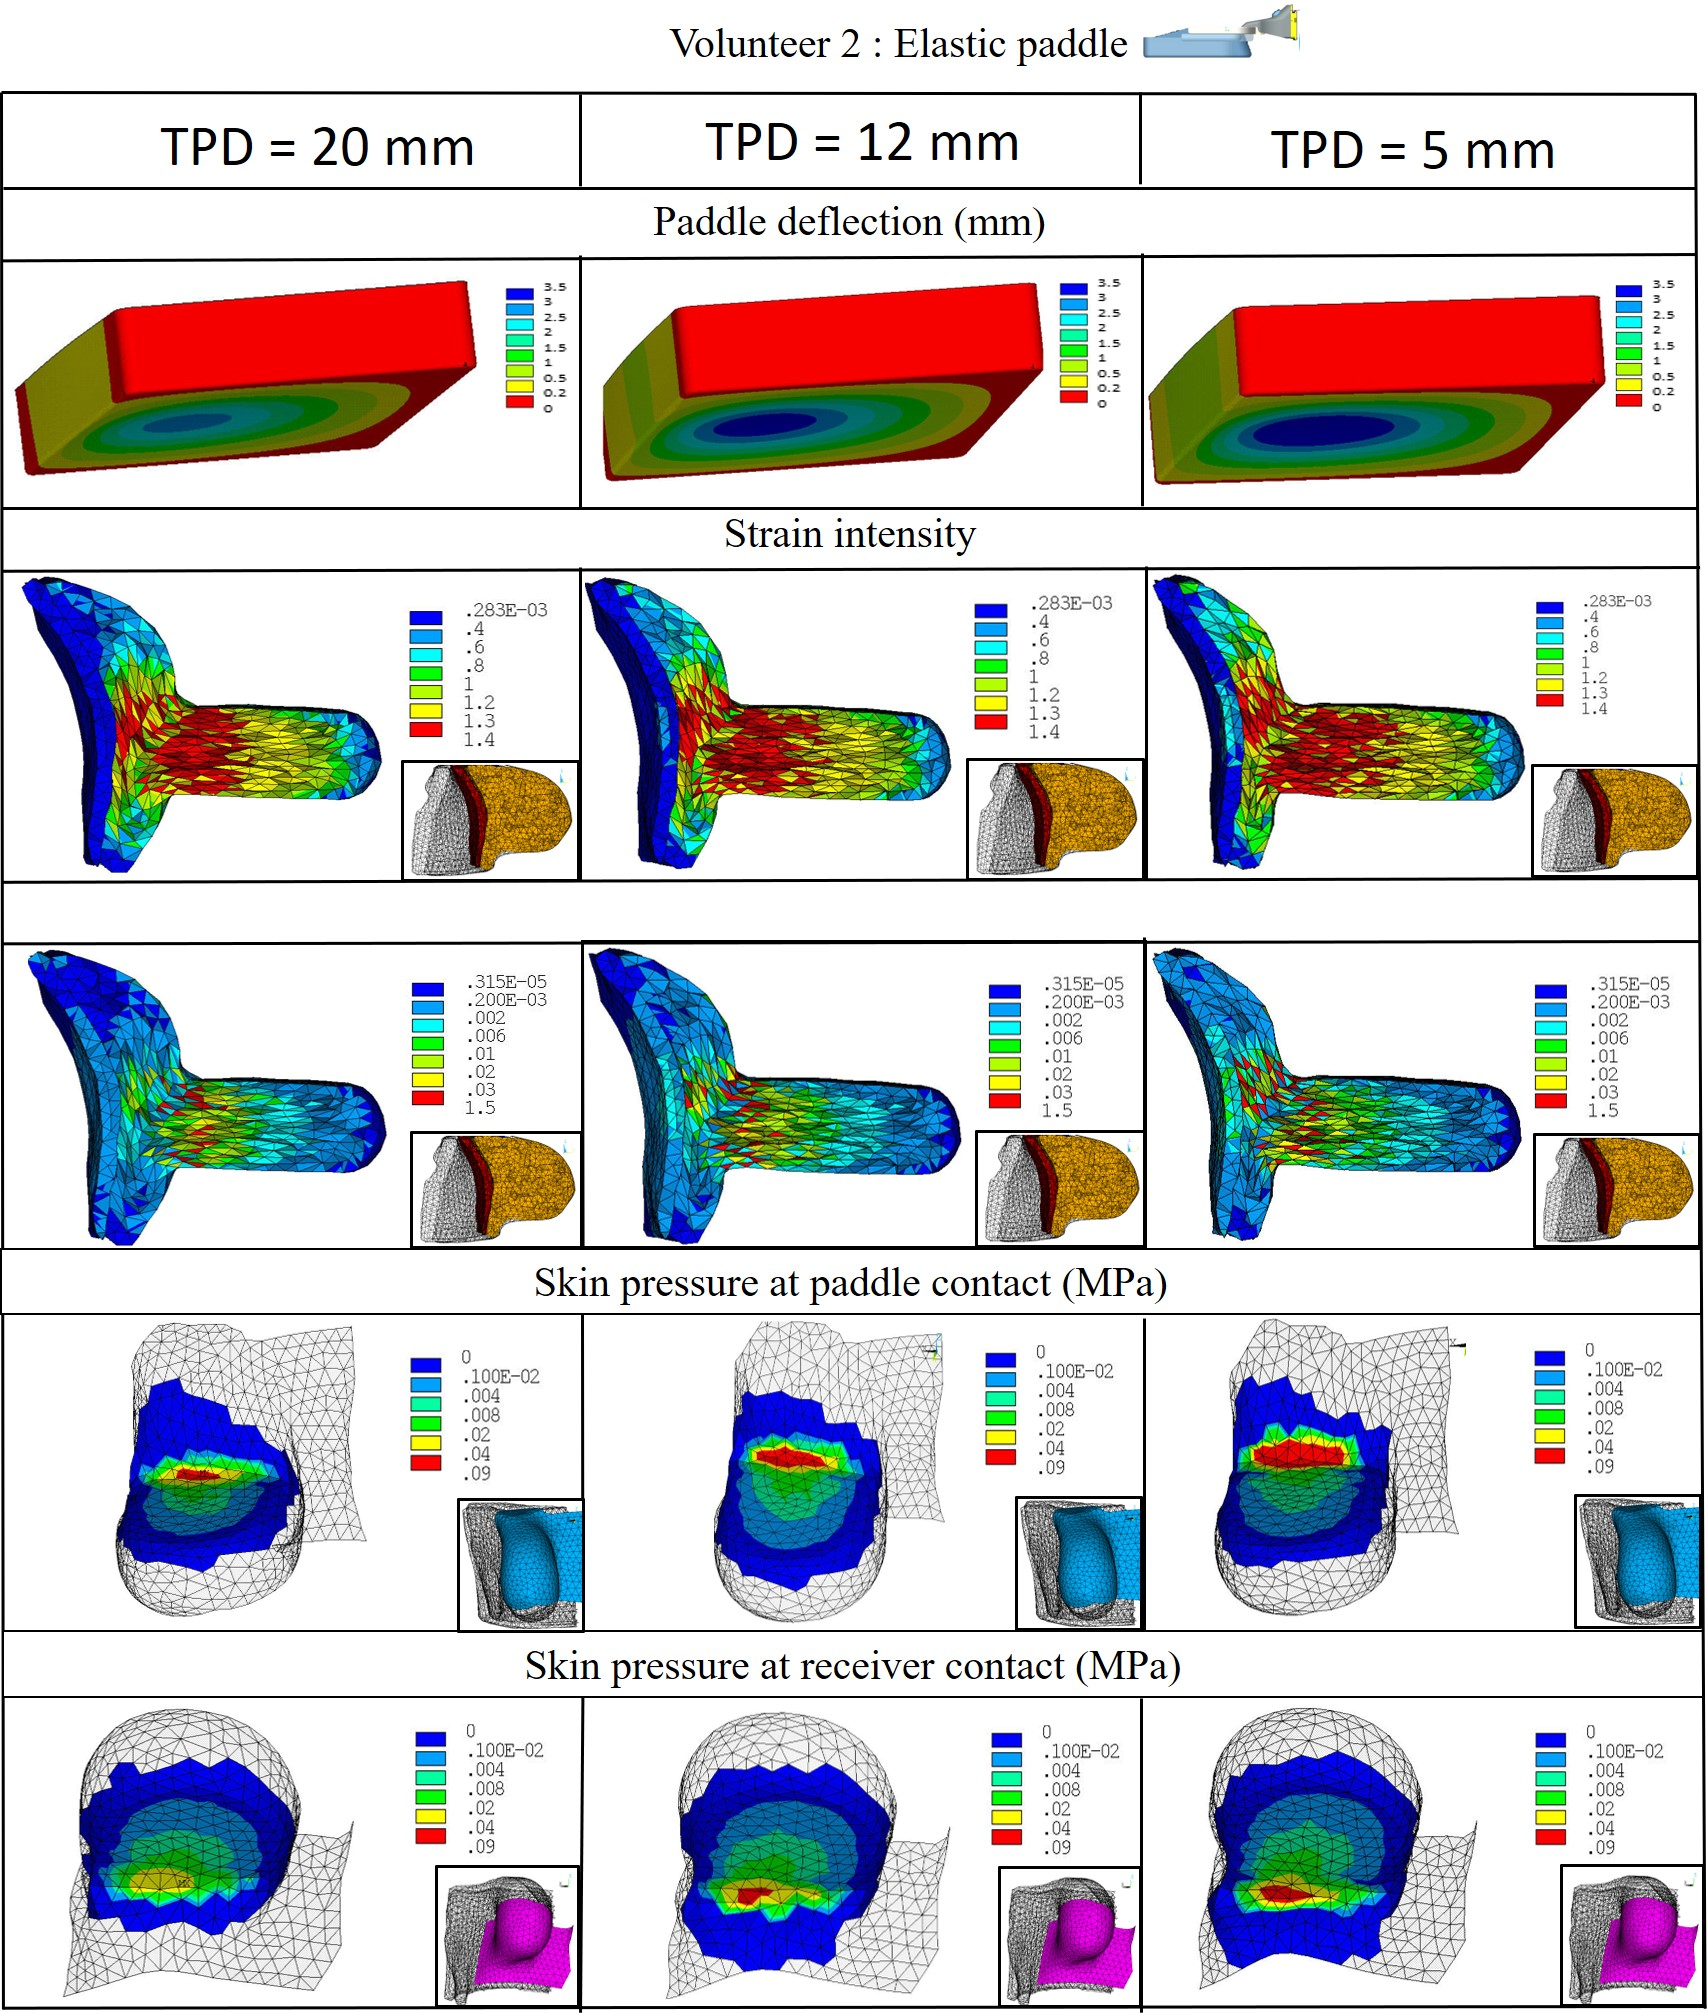
\includegraphics[width=0.9\textwidth,keepaspectratio]{figures/elasticpaddleresults.jpg} 
\caption{Stress, strain and contact pressure distribution for a variable thoracic cage to paddle distance (TPD).}\label{fig:elasticpaddle}
\end{figure}


Due to the paddle elasticity, the breast thickness slightly varies, with a maximal deflection equal to $3.5\ mm$ (Figure \ref{fig:elasticpaddle} first line). A very small difference between the maximal paddle deflection  $(\sim 1\ mm)$ was observed within the previous three compressions. Thus, image quality or AGD were not significantly impacted by the breast thickness variation. However, the wider the space between the chest wall and the compression paddle, the fewer breast tissues in the projected mammography image. In a standard framework, the technologist will include as much breast tissues as possible in order to reduce the risk of missing a suspicious lesion.

When looking at the strain distribution, one can see that, when the compression paddle is positioned closer to the chest wall, the juxtathoracic soft tissue undergoes higher deformation resulting also in a higher stress intensity. Concerning the skin surface pressure distribution, the highest intensities $ (\sim 90\ kPa)$ are always concentrated in the juxtathoracic area. However, for a thorax to paddle distance equal to $33\ mm$, the area corresponding to the high pressure is considerably larger. This means that a significant part of the total force was  used to compress the tissues in the juxtathoracic area only, which may increase the patient discomfort.

\section{Discussion and conclusion}\label{section:compressionfem:conclusion}

In this chapter, the breast compression was simulated using three paddles models, the rigid, flex and elastic models. In order to comply with the compression mechanics as described in literature, an update of the tissues constitutive models was needed. Appling the Gent form of strain-energy potential, instead of the Neo-Hookean form, allowed to obtain compression force magnitudes comparable with the real subject data. However, when the same law is used to perform the multi-loading gravity simulations, the breast deformations in supine and prone configurations are over-constrained. We found that, with a larger value of $J_m$ parameter, the Gent model may improve the breast geometry estimates obtained with a Neo-Hookean model.
In conclusion, the estimated value of $J_m$ does not characterize the subject-specific mechanical properties and gives only an estimation of a standard behaviour.  Our second study shows that, to obtain a proper estimation of parameter $J_m$, more information like the paddle position with respect to the breast volume is needed. 

The patient comfort (measured as strain and stress) as well as the image quality (measured as SNR, SDNR ) and AGD were compared for breast compression with rigid and flex paddles. The results from the two volunteers were analysed. The compression simulations indicate that, for the smallest breast, there is no significant difference for the patient perceived pain when using the rigid or the flex paddles. We did not observe any statistically significant difference in SNR or SDNR for microcalcification of any size. Therefore, our results suggest that using a flex paddle should not significantly impact image quality and delivered dose in small breasts and should not reduce significantly the perceived pain.   
For the largest breast, our simulations indicate that using a flex paddle may reduce the maximal pressure intensity on the skin surface by about 30\% compared to the rigid paddle. The tissues deformation is more uniformly distributed inside the breast volume, and the highest deformation occurs in the middle breast region corresponding to the supposed location of dense tissues. Moreover, our simulations have shown that the flex paddle has no significant impact on the average glandular dose and improves image quality compared to the rigid paddle. 

The impact of paddle positioning on patient comfort and image quality was also addressed. Three paddle positions with respect to the chest wall were studied using the elastic compression paddle. Even if a variable breast thickness is obtained due to the paddles deflection, the variations are too small ($\sim 1mm$) to impact the AGD or the resulting image quality in terms of the SNR or SDNR. However, some authors reported a risk of excluding some retromammary tissues from the imaged area, and consequently information on small posterior cancerous lesions may be lost. In terms of patient comfort, the simulations have shown that the high pressure are always localized in the juxtathoracic areas. When the paddle is too close to the chest wall, the compression force is mostly dissipated on this narrow area resulting in very high pressures compared to the skin pressure over the breast ($90kPa\ vs\ 10kPa$).
